\documentclass[convert]{standalone}

\usepackage{tikz}
\pagestyle{empty}

\begin{document}
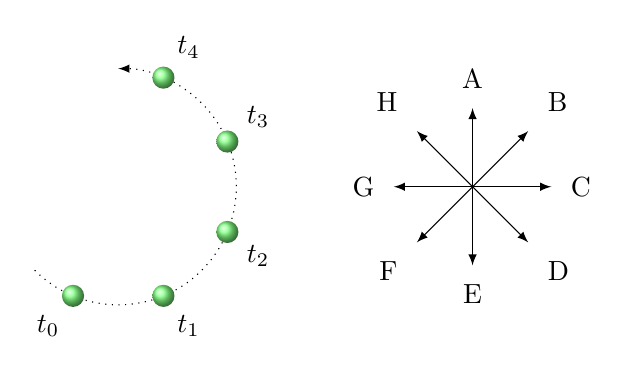
\begin{tikzpicture}[> = latex]

	% Definitions
	
	\def\R{1.5}		% Radius of circular motion
	
	% Draw circular path
	
	\draw [dotted, ->] (-135 : \R) arc (-135 : 90 : \R);
	
	% Draw ball
	
	\foreach \Q/\n in {-112.5/0, -67.5/1, -22.5/2, 22.5/3, 67.5/4}
		\draw [ball color = green!50, draw = none] (\Q : \R) circle (4 pt) node [label = {\Q : $t_\n$}] {};
		
	% Draw direction labels
	
	\foreach \Q/\s in {90/A, 45/B, 0/C, -45/D, -90/E, -135/F, -180/G, -225/H}
		\draw [->] (3 * \R, 0) -- ++ (\Q : 1) node [label = {\Q : \s}] {};
	
\end{tikzpicture}
\end{document}